\documentclass[12pt,a4paper]{article}
\usepackage[utf8]{inputenc}
\usepackage[T1]{fontenc}
\usepackage[dutch]{babel}
\usepackage{amsmath}
\usepackage{amsfonts}
\usepackage{amssymb}
\usepackage{graphicx}
\usepackage{wrapfig}
\usepackage{enumitem}
\usepackage{hyperref}
\usepackage{gensymb}
\usepackage{siunitx}

\newcommand{\Luda}{\Big\Updownarrow}

\author{Estelle Severs, Matthias Kovacic}
\title{Afleidingen Natuurkunde}
\date{:)}
\begin{document}
    \maketitle
    \tableofcontents
    \newpage


    \section{Algemene afspraken rond dit document}


    \section{Algemene te kennen theorie}

    \subsection{Prefixen}
    \begin{center}
        \begin{tabular}{ | c | c | c | }
            \hline
            Prefix & Afkorting & Value      \\
            \hline
            Giga   & G         & $10^{9}$   \\
            Mega   & M         & $10^{6}$   \\
            Kilo   & k         & $10^{3}$   \\
            Hecto  & h         & $10^{2}$   \\
            Deka   & da        & $10^{1}$   \\
            Deci   & d         & $10^{-1}$  \\
            Centi  & c         & $10^{-2}$  \\
            Milli  & m         & $10^{-3}$  \\
            Micro  & $\mu$     & $10^{-6}$  \\
            Nano   & n         & $10^{-9}$  \\
            Pico   & p         & $10^{-12}$ \\
            \hline
        \end{tabular}
    \end{center}

    \subsection{Vectoren}
    Vergeet niet je vector altijd in componenten te splitsen! Vergeet ook niet op pijltjes boven de vectoren te zetten!

    \begin{itemize}
        \item \(A_x = A\cos\theta\) en \(A_y = A\sin\theta\)
        \item \(A = \sqrt{A_x^2 + A_y^2}\)
        \item \(\theta = \tan^{-1}(\frac{A_y}{A_x})\)
    \end{itemize}

    \subsubsection{Scalair product}
    De grote van deze vector vermenigvuldigd met de projectie van de andere vector op deze vector. Hieruit krijg je dus een scalar!!
    \[\textbf{A} \cdot \textbf{B} = AB \cos\theta\]

    \subsubsection{Vectorproduct}
    Dit product geeft altijd een vector loodrecht op beide vectoren. Deze uitkomst is te vinden met de rechterhandregel. Als je deze nog niet kent: zoekt es op op youtube ;)
    De grootte is te vinden met volgende formule:
    \[\textbf{A} \times \textbf{B} = AB\sin\theta\]

    \subsection{Pollevs}

    \begin{itemize}
        \renewcommand\labelitemi{--}
        \item Welke uitdrukking geeft het volume van een afgeknotte kegel?
        \begin{enumerate}
            [label=\alph*)]
            \item \(\pi(r_1 + r_2)\sqrt{h^2 + (r_1 - r_2)^2}\)
            \item \(2\pi(r_1 + r_2)\)
            \item \(\pi h(r_1^2 + r_1r_2 + r_2^2)\)
        \end{enumerate}
        \textit{Oplossing:} c, dit is de enige formule die een term gaat hebben tot de 3e macht en een volume is altijd van een macht 3.

        \item Voor welke van de volgende vectoren is de grootte van de vector gelijk aan een van de componenten van de vector?
        \begin{enumerate}
            [label = \alph*)]
            \item \(\vec{A} = 2\hat{\imath} + 5\hat{\jmath}\)
            \item \(\vec{B} = -3\hat{\jmath}\)
            \item \(\vec{C} = +5\hat{k}\)
            \item \(\vec{B} \text{ en } \vec{C}\)
        \end{enumerate}
        \textit{Oplossing:} c is het juiste antwoord. a kan niet omdat de grootte van de vector moet gelijk zijn aan de grote van de component. b kan niet omdat de grootte van een component niet negatief kan zijn. (na te kijken, not sure). Hieruit volgt dat d natuurlijk niet waar kan zijn.

        \item Welk van de volgende stellingen is juist, over het verband tussen \(\vec{A} \cdot \vec{B}\) en \((-\vec{A}) \cdot (-\vec{B})\)
        \begin{enumerate}
            [label=\alph*)]
            \item \(\vec{A} \cdot \vec{B} = -((-\vec{A})\cdot(-\vec{B}))\)
            \item als \(\vec{A} \cdot \vec{B} = AB\cos\theta \), dan is \((-\vec{A}) \cdot (-\vec{B}) = AB\cos(\theta + 180\degree)\)
            \item Zowel a als b is correct.
            \item Zowel a als b is fout.
        \end{enumerate}
        \textit{Oplossing:} d is het juiste antwoord.
        Of de vectoren nu in de positieve of negatieve richting staan, de hoek zal niet veranderen.
        De lengte van de vectoren zal ook gelijk blijven.

        \item Gegeven: twee vectoren $\vec{a}$ en $\vec{b}$, gelegen in het xy-vlak.
        Bepaal \(c = \vec{a} \times \vec{b}\)
        \begin{enumerate}
            [label=\alph*)]
            \item \(\vec{c} = - ab \sin(\pi/2 - \phi)\hat{k}\)
            \item \(\vec{c} = ab \cos(\phi)\hat{k}\)
            \item \(\vec{c} = ab \cos(\pi/2 - \phi)\)
            \item Geen van deze antwoorden is correct.
        \end{enumerate}
        \textit{Oplossing:} a is juist. De richting van de vector is dan -$\hat{k}$, het vectorproduct gebruikt een sinus om de grootte te bepalen en de hoek tussen $\vec{a}$ en $\vec{b}$ is 90$\degree$ - $\theta$
    \end{itemize}


    \section{Deel 1 - Mechanica}


    \section{Kinematica in 1 dimensie}
    2.1-2.6, 2.8-2.9

    \subsection{2.5: Formules bij constante versnelling}
    We nemen aan dat het initiële tijdstip in elk van deze formules altijd 0 is. \((t_{0} = 0)\).
    Vergelijking voor snelheid afleiden:
    \[\mathbf{a = \frac{dv}{dt} = constante}\]
    \begin{center}
	    $\Luda$ \[a dt = dv\]
	    $\Luda$ \[\int_{v_0}^{v} a \, dt = \int_{0}^{t} \,dv\]
	    $\Luda$\[v - v_0 = at\]
	    $\Luda$\[\mathbf{v = v_0 + at}\]
    \end{center}
    Vergelijking voor verplaatsing afleiden:
    \begin{center}
               \[v = \frac{dx}{dt}\]
	    $\Luda$\[dx = v dt\]
	    $\Luda$\[x - x_0 = \int_{0}^{t} v \, dt\]
	    $\Luda$\[x - x_0 = \int_{0}^{t} (v_0 + at) \, dt\]
	    $\Luda$\[x - x_0 = \int_{0}^{t} v_0 \, dt + \int_{0}^{t} at \, dt\]
	    $\Luda$\[\mathbf{x - x_0 = v_0t + a\frac{t^2}{2}}\]
    \end{center}
    Alternatieve vergelijking voor snelheid:
    \begin{center}
    	\[\bar{v} = \frac{v_0 + v}{2} \text{en} t = \frac{v - v_0}{a}\]
    \end{center}
    dan geldt voor de vergelijking van verplaatsing:
    \begin{center}
               \[x = x_0 + (\frac{v + v_0}{2})(\frac{v - v_0}{a})\]
	    $\Luda$\[x = x_0 + \frac{v^2 + v_0^2}{2a}\]
	    $\Luda$\[\mathbf{v^2 = v_0^2 + 2a(x - x_0)}\]
    \end{center}


    \section{Kinematica in twee of drie dimensies}
    3.7

    \subsection{Projectiel beweging: formules}
    \begin{figure}[h]
        \centering
        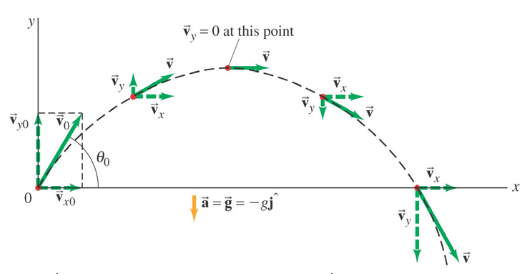
\includegraphics[width=0.7\linewidth]{projectiel}
        \caption{Er zal enkel een in de verticale component een versnelling aanwezig zijn. Hierdoor verandert de snelheid enkel in de verticale component.}
        \label{projectiel}
    \end{figure}
    \begin{table}[h]
        \centering
        \begin{tabular}{|c|c|}
            \hline
            \textbf{Horizontaal}     & \textbf{Verticaal}                        \\
            \hline
            \(a_x = 0\)              & \(a_y = -g\)                              \\
            \hline
            \(v_x(t) = v_{x0}\)      & \(v_y(t) = v_{y0} - gt\)                  \\
            \hline
            \(x(t) = x_0 + v_{x0}t\) & \(y(t) = y_0 + v_{y0}t - \frac{gt^2}{2}\) \\
            \hline
        \end{tabular}
    \end{table}


    \section{Dynamica: Newton's bewegingswetten}
    4.1-4.7

    \subsection{Eerste wet: inertie}
    Een lichaam in rust (of in eenparige rechtlijnige beweging) zal in rust (eenparige rechtlijnige beweging) blijven tenzij er een uitwendige resulterende kracht inwerkt.
    \[\sum_{i}\vec{F_i} = 0 \Rightarrow \vec{a} = 0\]

    \subsection{Tweede wet: versnelling}
    Een grotere kracht op een lichaam met massa m veroorzaakt een grotere versnelling: $a \sim F$

    Bij een dubbele massa 2m zal eenzelfde kracht slechts een versnelling a/2 veroorzaken: $a \sim \frac{1}{m}$

    \[\sum_{i} \vec{F_i} = \vec{F} = m\vec{a}\]

    \subsection{Derde wet: actie-reactie}
    Bij wisselwerking tussen twee lichamen is de kracht \(\vec{F_{21}}\) van lichaam 1 op lichaam 2 even groot en tegengesteld aan de kracht \(\vec{F_{12}}\) van lichaam 2 op lichaam 1.
    \[\vec{F_{12}} = -\vec{F_{21}}\]
    Deze krachten komen steeds in paren voor en werken op verschillende voorwerpen.

    \subsection{Gewicht - Gravitatie - Normaalkracht}
    Alle voorwerpen nabij het aardoppervak vallen met dezelfde versnelling $\vec{g}$.
    \[\text{Gravitatiekracht: } \vec{F_G} = m\vec{g}\]


    \section{De wetten van Newton: wrijving, cirkelbeweging, weerstandskrachten}

    \subsection{Delen in de Giancoli}
    5.1-5.3, 5.5-5.6
    
    \subsection{Wrijvingskrachten}
    Voorwerpen in een ERB duren niet oneindig, de oorzaak hiervan is de wrijvingskracht. Dit is weerstand wanneer een voorwerp
    over het oppervlak van een ander voorwerp beweegt. Deze wrijvingskracht is proportioneel afhankelijk van de normaalkracht
    op een voorwerp $F_{fr} \sim F_{n}$.  De everedigheidsconstante hangt af van de soort wrijvingskracht op een voorwerp.\\
    
    \newpage
    
    Er zijn twee soorten wrijvingskrachten:
    \begin{enumerate}
            [label=\alph*)]
            \item Kinetische wrijvingskracht
            \item Statische wrijvingskracht
        \end{enumerate}
        
    De nettokracht op een voorwerp is gegeven als volgt:
    
    $$ F_{net} = F_{A} -  F_{fr} $$
    
     \begin{figure}[h]
        \centering
        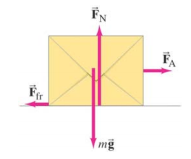
\includegraphics[width=0.3\linewidth]{papierdoos}
        \caption{Verduidelijkende figuur bij wrijvingskrachten}
        \label{papierdoos}
    \end{figure}    
        
    Kinetische wrijvingskracht is de wrijvingskracht die inwerkt op een voorwerp als het voorwerp in beweging is.    
    De grootte van deze wrijvingskracht is afhankelijk van de kinetische wrijvingscoëfficient $\mu_{k}$:
    
   $$ F_{k} = \mu_{k}F_{n} $$
   
   Statische wrijvingskracht is de wrijvingskracht die inwerkt op een voorwerp als het voorwerp nog niet in beweging is.
   De grootte van deze wrijvingskracht is afhankelijk van de statische wrijvingcoëfficient $\mu_{s}$:
   
   $$F_{s} \leq \mu_{s}F_{n}$$
   
   Belangrijk is op te merken dat als het voorwerp in rust staat, de volgende gelijkheid geldt:
   
   $$\vec{F_{s}} = -\vec{F_{A}}$$
   
   In het algemeen is het moeilijker een voorwerp in beweging te krijgen dan het verder te laten bewegen en is dus $\mu_{s} > \mu_{k}$
   
   \subsection{Weerstand en eindsnelheid}
   Als het voorwerp zich doorheen een medium (of fluïda) beweegt, is de wrijvingskracht afhankelijk van de snelheid van het voorwerp.
   Voor relatief kleine voorwerpen met lage snelheid geldt:
   
   $$ \vec{F_{d}} = -b\vec{v} $$
   
   waarbij $b$ een factor is die afhangt van de grootte/vorm van het voorwerp en de viscositeit (of stroperigheid)
   van de vloeistof.
   
   In evenwicht geldt dat de eindsnelheid van een voorwerp gegeven wordt door:
   
   \begin{center}
   	 \[F_{net} = 0\]
	  $\Luda$\[mg - bv_{t} = 0\]
	  $\Luda$\[v_{t} = \frac{mg}{b}\]
    \end{center}	  

    \subsection{Kinematica van de cirkelbeweging}
    Als een voorwerp in een cirkel beweegt, verandert de richting van de snelheid constant. Dit wilt dus zeggen dat:
    
    $$ \vec{a} \neq 0$$
    
    We kunnen de richting als volgt afleiden:
    
    \begin{center}
    	\[\vec{a} = \lim_{\Delta t\to\infty} = \frac{\Delta \vec{v}}{\Delta t} = \frac{d\vec{v}}{dt}\]
    	$\Luda$\\
    	Als $\Delta t$ infinitesimaal klein wordt is $\Delta \vec{v}$ infinitesimaal klein\\
    	$\Luda$\[\Delta\vec{v} \perp \vec{v}\]
    	$\Luda$\[\vec{a} \perp \vec{v}\]
    	$\Luda$\\ 
    	$\vec{a}$ wijst naar het middelpunt van de cirkel.
    \end{center}
    
    De grootte leiden we als volgt af:
    
    \begin{center}
    	\[\vec{a} = \lim_{\Delta t \to 0} = \frac{\Delta \vec{v}}{\Delta t} = \frac{d\vec{v}}{dt}\]
    	$\Luda$\\ Uit de figuur leiden we gelijkvormige driehoeken $1$ en $2$ af
	    	\begin{figure}[h]
	        		\centering
	       		 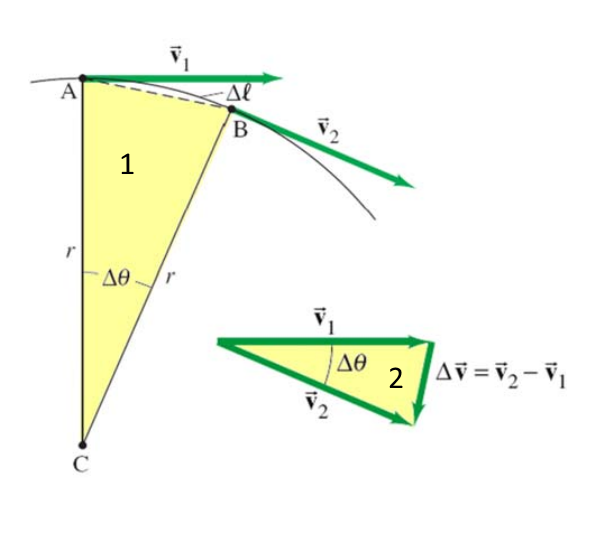
\includegraphics[width=0.6\linewidth]{cirkel}
	       		 \caption{Gelijkvormige driehoeken bij afleiding grootte van de versnelling van een cirkelbeweging}
	        		\label{cirkel}
	    	\end{figure}
	$\Luda$\[\frac{\Delta v}{v} \sim \frac{\Delta l}{r}\]
	$\Luda$\[\Delta v \sim \frac{v\Delta l}{r}\]	    	
	We zien nu dat:
	\[a_{r} = \lim_{\Delta t\to\infty} \frac{\Delta v}{\Delta t}\]
	$\Luda$\[a_{r} = \lim_{\Delta t \to 0} \frac{v}{r}\frac{\Delta l}{\Delta t}\]
	$\Luda$\[a_{r} = \frac{v}{r} \lim_{\Delta t \to 0} \frac{\Delta l}{\Delta t}\]
	$\Luda$\[a_{r} = \frac{v^{2}}{r}\]
    \end{center}
    
    We kunnen ook met behulp van volgende begrippen de snelheid van een voorwerp in een cirkelbeweging afleiden:
    \begin{enumerate}
    	\item de periode $T$ = tijd nodig voor 1 omwenteling
    	\item de frequentie $f$ = aantal omwentelingen per seconde (in Hertz)
    \end{enumerate}
    
    We zien dan dat $T = \frac{1}{f}$ en dat:
    
    \begin{center}
    	\[v = \frac{2\pi r}{T}\]	
    \end{center}
    
    \subsection{Dynamica van de cirkelbeweging}
    Er is een kracht nodig om een voorwerp op een cirkelbaan te houden, dit is de centripetale kracht. Deze kracht wijst altijd naar het middelpunt
    van de cirkel en zorgt voor een centripetale versnelling. 
    
    $$ \sum F_{R} = ma_{r} = m\frac{v^{2}}{r} $$ 
    
    Als de centripetale kracht wegvalt, zal door inertie (eerste wet van Newton), het voorwerp gewoon rechtdoor bewegen in plaats van op de cirkelbaan te blijven. 
    De snelheid van een voorwerp kan ook veranderen. Dan heeft de versnelling twee componenten: de radiale component en de tangentiële component. Deze componenten
    kunnen worden gezien als componenten voor de totale versnelling:
    
    \begin{enumerate}
    	\item $a_{r} = \frac{v^{2}}{r}$
    	\item $a_{tan} = \frac{dv}{dt}$
    \end{enumerate}
    
    Dan is de totale versnelling gelijk aan:
    
    $$ a = \sqrt{a_{tan}^{2} + a_{r}^{2}} $$ 
    
    \begin{figure}[h]
    	\centering
	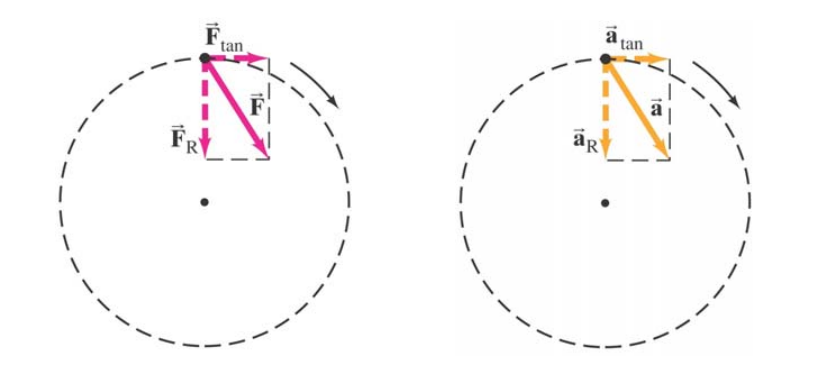
\includegraphics[width=0.6\linewidth]{cirkel_versnelling}
    	\caption{Radiale en tangentiële versnelling bij een cirkelbeweging}
        	\label{cirkel_versnelling}
    \end{figure}

    \section{De zwaartekracht en de synthese van Newton}

    \subsection{Delen in Giancoli}
    6.1-6.4, 6.6

    \subsection{De wet van de universele zwaartekracht}
    Elk paar van voorwerpen oefent een kracht uit op elkaar. Zo oefent ook de Aarde een kracht uit op andere voorwerpen (vb. de maan). 
    Uit de tweede wet van Newton zien we dat de kracht evenredig is met de massa (1). Uit de derde wet van Netwon
    zien we dan ook dat de kracht evenredig is met de massa van de aarde (2). Uit experimenten halen we ook dat de kracht
    omgekeerd evenredig is met het kwadraat van de afstand tussen de twee voorwerpen (3). 
    
    \begin{enumerate}
    	\item $F \sim m_{voorwerp_{A}}$
    	\item $F \sim m_{voorwerp_{B}}$
    	\item $F \sim \frac{1}{r^{2}}$
    \end{enumerate}
    
    Als we deze 3 eigenschappen combineren vinden we dat de kracht tussen de twee voorwerpen gegeven wordt door:
    
    $$ F \sim \frac{m_{A}m_{b}}{r^{2}} $$

    Elk deeltje in het universum trekt elk ander deeltje aan met een kracht die recht everedig is met het product van hun massa's en omgekeerd
    evenredig is met het kwadraat van hun afstand. Voor de zwaartekracht is de evenredigheidsconstante $G$:
    
    $$ G = 6.673 \times 10^{-11} \frac{Nm^{2}}{kg^{2}} $$ 
    
    Waaruit volgt dat de zwaartekracht $F_{g}$ gedefinieerd is als:
    
    $$ F_{g} = G \frac{m_{A}m_{b}}{r^{2}} $$ 
    
    Belangrijk is te weten dat dit enkel geldt voor puntmassa's! Voor een symmetrische bol of schil, 
    doen we alsof alle massa in één punt zit.
    
    \subsection{Zwaartekracht nabij het oppervlak}
    Als een massa zicht op een hoogte $h$ boven het aardoppervlak bevindt en de straal van de aarde is $R_{a}$, dan is de zwaartekracht op dat voorwerp:
    
    $$ F_{a} = G\frac{mM_{a}}{(R_{a} + h)^{2}} \sim G\frac{mM_{a}}{R_{a}^{2}}$$
    
    We kunnen nu de valversnelling afleiden:
    
    $$ F_{a} = ma $$
    $$\Luda$$
    $$ F_{a} = mg $$
    $$\Luda$$
    $$ F_{a} = G\frac{M_{a}}{R_{a}^{2}} $$
    $$\Luda$$
    $$ g = 9.81 \frac{m}{s^{2}} $$
    
    Aangezien dit berekent is op $h = 0$, kan dit echter afwijken afhankelijk van $h$ als $0 \leq h$. 
    
    \subsection{Satellieten}
    Uit de eerste wet van Newton weten we dat een satelliet zondere kracht rechtdoor zou bewegen. Er werkt echter een kracht in
    op de satelliet, namelijk de gravitatiekracht. We weten dus dat de kracht die inwerkt op de satelliet, de gravitatiekracht, de satelliet
    op zijn baan houdt:
    
    $$ F_{a} = ma $$
    $$\Luda$$
    $$ G\frac{mM_{a}}{r^{2}} = m\frac{v^{2}}{r} $$ 
    $$\Luda$$
    $$ v = \sqrt{\frac{GM_{a}}{r}}$$
    $$\Luda$$
    $$ v = \sqrt{\frac{GM_{a}}{R_{a} + h}} $$
    
    \subsection{Het gravitatieveld}
    Het gravitatieveld is een manier op de impact van de gravitatie in algemene termen weer te geven voor eender welk punt. Het kan gedefinieerd worden met behulp
    van volgende afleiding.
    
    $$ \vec{F_{g}} = -m\vec{a}$$
    $$\Luda$$
    $$ \vec{F_{g}} = -mG\frac{M_{a}}{r^{2}}\vec{u_{r}}$$
    $$\Luda$$
    $$ \vec{F_{g}} = -mg\vec{u_{r}}$$
    $$\Luda$$
    $$ \vec{F_{g}} = m\vec{g}$$
    $$\Luda$$
    $$ \vec{g} = \frac{\vec{F_{g}}}{m}$$
    
    We zien nu dat een massa $m$ die geplaatst wordt op een punt waar het veld gelijk is aan $\vec{g}$ een kracht ondervindt:
    
    $$ \vec{F_{g}} = m\vec{g}$$ 

    \section{Arbeid en energie}

    \subsection{Delen in Giancoli}
    7.1, 7.3-7.4 (+14.1)


    \section{Behoud van energie}

    \subsection{Delen in Giancoli}
    8.1-8.3, 8.5, 8.8


    \section{Impuls}

    \subsection{Delen in Giancoli}
    9.1-9.2 (+36.11)


    \section{Rotatie}
    10.1, 10.4, 10.8


    \section{Impulsmoment}

    \subsection{Delen in Giancoli}
    11.3-11.4, 11.6
    \newpage


    \section{Deel 2 - Elektriciteit}


    \section{Elektrische velden}

    \subsection{Delen in Giancoli}
    21.1-21.2, 21.4-21.11, 21.13


    \section{De wet van Gauss}

    \subsection{Delen in Giancoli}
    22.1-22.3


    \section{Elektrische potentiaal}

    \subsection{Delen in Giancoli}
    23.1-23.9


    \section{Condensatoren en diëlektrica}

    \subsection{Delen in Giancoli}
    24.2-24.6


    \section{Elektrische stroom en weerstand}

    \subsection{Delen in Giancoli}
    25.1-25.6, 25.8-25.9 (+40.7-40.10)


    \section{Gelijkstroomschakelingen}

    \subsection{Delen in Giancoli}
    26.2-26.5, 26.7
    \newpage


    \section{Deel 3 - Magnetisme}
    Dit is geen deel van het vak in het eerste jaar, maar zal je misschien van pas komen in het tweede jaar ;).
\end{document}